\section{Auswertung}
\label{sec:Auswertung}

\subsection{Charakteristik des Zählrohrs}
  Um die Charakteristik des Zählrohrs zu untersuchen, wird eine $\beta$-Quelle vor das 
  Fenster des Zählrohrs gestellt und unter Variations der Betriebsspannung U die 
  Zählrate gemessen. Diese sind in folgender Grafik \ref{fig:plot} dargestellt.
  \begin{figure}
    \centering
    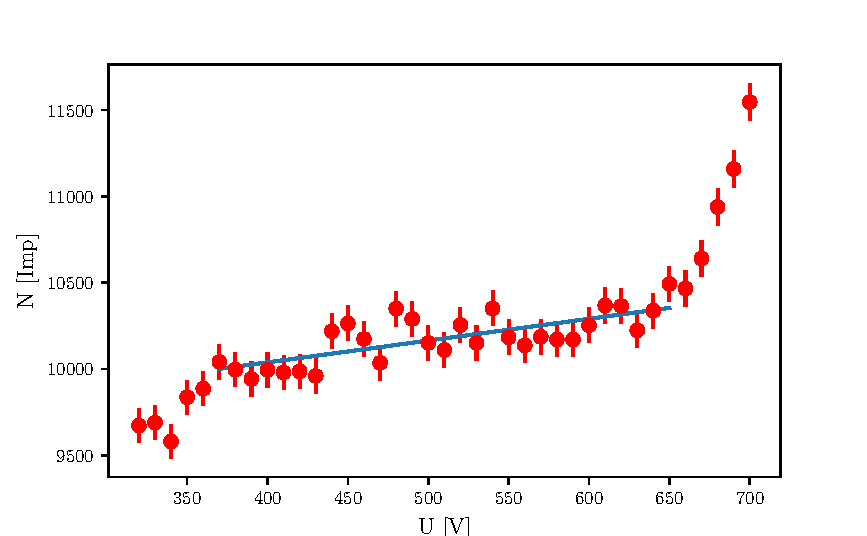
\includegraphics{plot.pdf}
    \caption{Plot.}
    \label{fig:plot}
  \end{figure}
  Das Plateau erstreckt sich circa von$370 V$ bis $640 V$ und wurde mit einer linearen 
  Regression $f = a\cdot V + b$ gefittet. Die daraus resultierende Plateau-Steigerung 
  beträgt $1.262 \pm 0.218$ \% pro 100 V. Für einen Reibungslosen Ablauf der folgenden 
  Versuchsteile kann eine Spannung von 500 V gewählt werden.

\subsection{Totzeitbestimmung anhand eines Oszilloskopes}

\subsection{Totzeitbestimmung anhand der Zwei-Quellen-Methode}
  Für die Totzeitbestimmung wurden 120 Sekunden lang zunächst die Impulse $N_1$ einer einzelnen
  $^{204}$Tl-Quelle gemessen, dann die Impulse $N_{1+2}$ von zweien und dann diejenigen der 
  Letzeren. Die Totzeit kann näherungsweise durch die in der Theorie hergeleitete Formel 
  \begin{equation*}
  T \approx \dfrac{N_1+N_2-N_{1+2}}{2N_1N_2}= 8.1566 \cdot 10^{-9} s
  \end{equation*}
  bestimmt werden.
